\documentclass[norsk]{beamer}
 
\usepackage[T1]{fontenc}
\usepackage{textcomp,pdfpages}
\usepackage{babel}

\usepackage{amsmath, amsfonts, epsfig, xspace}
\usepackage{pstricks,pst-node}
\usepackage{multimedia}
\usepackage{beamerthemesplit}
\usepackage[absolute, overlay]{textpos}
\usepackage{listings}

\usepackage{color}
 
\definecolor{dkgreen}{rgb}{0,0.6,0}
\definecolor{gray}{rgb}{0.5,0.5,0.5}
\definecolor{mauve}{rgb}{0.58,0,0.82}

\lstset{
  language=java,
  aboveskip=3mm,
  belowskip=3mm,
  showstringspaces=false,
  columns=flexible,
  basicstyle={\tiny\ttfamily},
  numberstyle=\tiny\color{gray},
  keywordstyle=\color{blue},
  commentstyle=\color{dkgreen},
  stringstyle=\color{mauve},
  breaklines=true,
  breakatwhitespace=true,
  tabsize=2
}
 


\usetheme{bekk}


\author{Aslak Johannessen \\ aslakjo@bekk.no  @aslakjo}

\title[Scala]{Actors}
\subtitle[]{Scala -actors}
\institute{BEKK Consulting AS}


\begin{document}

\maketitle

\begin{frame}{Scala quiz}
  \begin{content}
    Oppgave: Lag et quizlag og implementer det som en actor\\
    
    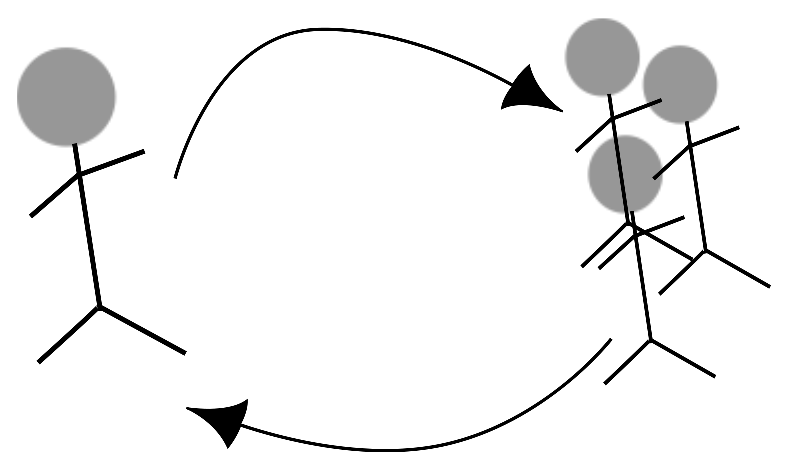
\includegraphics[scale=0.9]{quizlag}
  \end{content}
\end{frame}

\begin{frame}{Scala quiz}
  \begin{content}
    Quiz p� vanlig m�te, med en liten vri\\
    \center
    1. Be om et sp�rsm�l og f� sp�rsm�l\\
    \includegraphics[scale=0.6]{quiz-sporsmalsvar}\\
    2. Svar p� sp�rsm�let og f� vite om det er riktig
  \end{content}
\end{frame}


\begin{frame}{Actors - hva er greia}
  \begin{content}
    Wikipedia: \\
    \begin{quotation}In computer science, the Actor model is a mathematical model of concurrent computation that treats "actors" as the universal primitives of concurrent digital computation: in response to a message that it receives, an actor can make local decisions, create more actors, send more messages, and determine how to respond to the next message received. The Actor model originated in 1973. It has been used both as a framework for a theoretical understanding of concurrency, and as the theoretical basis for several practical implementations of concurrent systems.
    \end{quotation}
  \end{content}
\end{frame}

\begin{frame}{Actors - hva er greia}
  \begin{content}
    Wikipedia: \\
    \begin{quotation}... \emph{concurrent computation} ... \emph{in response to a message that it receives, an actor can make local decisions ... and        determine how to respond to the next message received.}  \emph{The Actor model originated in 1973.} ...
    \end{quotation}
  \end{content}
\end{frame}


\begin{frame}[fragile]{Actors - eksempler eksempler}
  \begin{content}
    \begin{lstlisting}
      case class Tick
      
      class Counter extends Actor {
        private var counter = 0

        def receive = {
          case Tick =>
            counter += 1
            println(counter)
        }
      }
    \end{lstlisting}
  \end{content}
\end{frame}

\begin{frame}{Actors - in action}
  \begin{content}
    \centering
    1. MoreQuestions(new Team(``lag en''))\\
    2. Question(``Ping'', Nil)\\
    \begin{columns}
      \column{.1\textwidth}
        Server
      \column{.5\textwidth}
        \includegraphics[scale=0.5]{quiz-sporsmalsvar}
      \column{.1\textwidth}
        Lag
    \end{columns}
    3. Answer(question, ``pong'')\\
    4. Correct()
  \end{content}
\end{frame}

\begin{frame}[containsverbatim]{Actors - in action}
  \begin{content}
    \centering
    \begin{lstlisting}
      case class MoreQuestions(val team:Team)
      case class Question(val question:String, val content:Any)
    \end{lstlisting}
    \begin{columns}
      \column{.1\textwidth}
        Server
      \column{.5\textwidth}
        \includegraphics[scale=0.5]{quiz-sporsmalsvar}
      \column{.1\textwidth}
        Lag
    \end{columns}
    \begin{lstlisting}
      case class Answer(val team:Team, val question:Question, val answer:Any)
      case class Correct extends Verdict
    \end{lstlisting}
  \end{content}
\end{frame}

\begin{frame}[containsverbatim]{Actors - in action}
  \begin{content}
    \begin{columns}
      \column{.2\textwidth}
        \includegraphics[scale=0.3]{quiz-sporsmalsvar}
      \column{.8\textwidth}
        \begin{lstlisting}
          val question = (remote !! MoreQuestions(team)).get.asInstanceOf[Question]
          remote !! new Answer( team, question, giveAnswer(question) )

          def giveAnswer(quiestion: Question)={
            question match {
              case x@Question("Ping", "") =>  "pong"
            }
          }
        \end{lstlisting}
    \end{columns}
  \end{content}
\end{frame}

\kontrast{Oppgave}

\begin{frame}[plain]
  \begin{centering}
    \includegraphics[height=11em]{bekk}
    \\\vspace{2em}\hfill\\
    \small
    \includegraphics[height=1em]{bekk-logo}
    \\\vspace{.4em}\hfill\\
    \fontsize{8}{8}
    \selectfont
    \textbf{Aslak Johannessen}\\
    Senior Consultant\\
    982 19 249 \\
    aslakjo@bekk.no\\
    \vspace{.3em}\hfill\\
    \fontsize{1}{1}
    \selectfont
    BEKK CONSULTING AS\\
    SKUR 39, VIPPETANGEN. P.O. BOX 134 SENTRUM, 0102 OSLO, NORWAY. WWW.BEKK.NO\\
  \end{centering}
\end{frame}

\end{document}
